%! TEX root = ../symbolic.tex

\chapter{Preliminarii}

\section{Introducere și motivație}

Articolul își propune să introducă o metodă prin care, folosind
învățarea automată, să se genereze expresii matematice de diverse
complexități și forme. Utilizarea acestor expresii este, de exemplu,
pentru rezolvarea problemelor matematice care necesită, din motive
teoretice, căutarea unor soluții într-un spațiu foarte mare.

Mai mult decît atît, însăși problema generării expresiilor simbolice
este una complicată pentru rețele neuronale, iar abordarea din articolul
\cite{lample2019deep} pe care îl prezentăm este una specifică traducerilor
automate sau a procesării limbajului natural (NLP).

Autorii remarcă faptul că tehnicile folosite în NLP pot fi utile și
în cazul expresiilor matematice simbolice. Dacă sistemele de tip
\emph{computer algebra} de obicei rezolvă probleme matematice prin algoritmi
foarte sofisticați, oamenii lucrează prin identificarea tiparelor în
expresiile matematice. Nicio rețea neuronală existentă în prezent nu a
fost folosită pentru identificarea tiparelor în expresii matematice,
însă.

%%%%%%%%%%%%%%%%%%%%%%%%%%%%%%%%%%%%%%%%%%%%%%%%%%%%%%%%%%%%%%%%%%%%%%

\section{Expresii matematice prin arbori sintactici}

Autorii propun utilizarea unei metode de traducere de tip \emph{sequence to %
sequence} (seq2seq, pe scurt), descrisă cu tot cu implementare în Python
în \cite{chollet}. Pentru aceasta, expresiile matematice sînt descompuse
folosind arbori de sintaxă, iar reprezentarea lor se face folosind
așa-numita \emph{formă poloneză} cu prefix. Astfel, expresia scrisă în 
mod clasic prin:
\[
    2 + 3 \cdot (5 + 2)
\]
va fi descrisă în notația poloneză prin \texttt{[+ 2 * 3 + 5 2]}, iar
prin arbore binar în forma din figura \ref{fig:mat-polish1}.

\begin{figure}[!htbp]
    \centering
    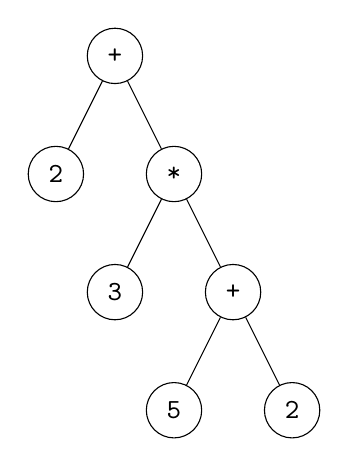
\begin{tikzpicture}[
        every node/.style = {minimum width = 2em, draw, circle},
        ]
        \node {\texttt{+}}
            child {node {\texttt{2}}}
            child {node {\texttt{*}}
                child {node {\texttt{3}}}
                child {node {\texttt{+}}
                    child {node {\texttt{5}}}
            child {node {\texttt{2}}}}};
    \end{tikzpicture}
    \caption{Arbore binar pentru expresia \texttt{[+ 2 * 3 + 5 2]}}
    \label{fig:mat-polish1}
\end{figure}

Similar se pot coda și expresii mai complicate, precum, de exemplu (v.\ fig. \ref{fig:arbore-pder}):
\[
    \frac{\partial^2 u}{\partial x^2} - \dfrac{1}{c^2} \frac{\partial^2 u}{\partial t^2}.
\]


\begin{figure}[!htbp]
    \centering
    \begin{tikzpicture}[
        every node/.style = {minimum width = 2em, draw, circle},
        ]
        % \node {-}
        %     child {node {$\partial$}
        %         child {node {$\partial$} child {node {$u$}}

    \end{tikzpicture}
    \caption{Arbore binar pentru expresia %
    $ \dfrac{\partial^2 u}{\partial x^2} - \dfrac{1}{c^2} \dfrac{\partial^2 u}{\partial t^2}$}
    \label{fig:arbore-pder}
\end{figure}
